%File: wmhs_drift_attribution_aaai.tex  (AAAI-26 AuthorKit, anonymous submission mode)
\documentclass[letterpaper]{article} % DO NOT CHANGE THIS
\usepackage[submission]{aaai2026}  % DO NOT CHANGE THIS
\usepackage{times}  % DO NOT CHANGE THIS
\usepackage{helvet}  % DO NOT CHANGE THIS
\usepackage{courier}  % DO NOT CHANGE THIS
\usepackage[hyphens]{url}  % DO NOT CHANGE THIS
\usepackage{graphicx} % DO NOT CHANGE THIS
\urlstyle{rm} % DO NOT CHANGE THIS
\def\UrlFont{\rm}  % DO NOT CHANGE THIS
\usepackage{natbib}  % DO NOT CHANGE THIS AND DO NOT ADD ANY OPTIONS TO IT
\usepackage{caption} % DO NOT CHANGE THIS AND DO NOT ADD ANY OPTIONS TO IT
\frenchspacing  % DO NOT CHANGE THIS
\setlength{\pdfpagewidth}{8.5in} % DO NOT CHANGE THIS
\setlength{\pdfpageheight}{11in} % DO NOT CHANGE THIS
\pdfinfo{
/TemplateVersion (2026.1)
}
% Allowed additions
\usepackage{amsmath,amssymb,amsthm}
\usepackage{booktabs}
\usepackage{microtype}
\usepackage{xcolor}   % draft only: used by \todo; remove before the final version
\setcounter{secnumdepth}{1}

\newtheorem{proposition}{Proposition}
\newtheorem{definition}{Definition}
\newtheorem{assumption}{Assumption}
\newcommand{\todo}[1]{\textcolor{red}{[TODO: #1]}}
\newcommand{\E}{\mathbb{E}}
\newcommand{\rhat}{\hat r}
\DeclareMathOperator*{\supp}{supp}

\title{Attributing Performance Drift Under Deployment Feedback: When the Model Is One of the Mechanisms}
\author{Anonymous submission}
\affiliations{}

\begin{document}


\maketitle

\begin{abstract}
\todo{Write last. One paragraph: (1) monitoring detects drift but does not
explain it; (2) attribution methods decompose a performance change into
distribution-shift mechanisms via a cooperative game, but the game's value
function assumes mechanisms can be switched independently; (3) once a model is
deployed and acted upon, the post-deployment environment is a causal descendant
of the model, the model-mediated policy has no counterpart in the pre-deployment
environment, and the game is no longer well defined; (4) we redefine the
estimand with the model-mediated component as a policy, give identification and
partial-identification results, and show in simulation that the naive
decomposition attributes performative success to outcome-mechanism shift and
reverses the retraining decision.}
\end{abstract}

%==============================================================================
\section{Introduction}
\label{sec:intro}

\todo{Four paragraphs, about one page.}

\paragraph{P1: the monitoring gap.} A deployed clinical prediction model's
performance drops. Monitoring reports that it dropped, not why. Three
mechanisms are observationally consistent with the same degradation and demand
different responses: the patient population changed (covariate shift), the
outcome mechanism changed (biology, care pathways, coding and documentation),
or the model worked: high-risk patients were flagged, clinicians intervened,
outcomes improved, and the learned predictor-outcome relationship was
invalidated by its own success~\citep{lenert2019victims, sperrin2019explicit,
balcarcel2025feedback}.

\paragraph{P2: attribution exists and is solved for the exogenous case.}
\citet{zhang2023attributing} formulate performance-change
attribution as a cooperative game whose players are causal mechanisms and
quantify each mechanism's contribution as its Shapley value; \citet{budhathoki2021rootcauses} attribute distribution change to individual
mechanisms; \citet{cai2023disde} decompose a drop into $Y|X$ and $X$
terms; \citet{gordaliza2025causal} carry the framework into
medical imaging. \emph{We do not claim that nobody decomposes drift into
causal components.}

\paragraph{P3: the formulation breaks under deployment feedback.} The game
defines the value of a set of mechanisms as the performance that would have
been observed had only that set changed. This requires each mechanism to be
independently switchable between environments. Under deployment feedback the
post-deployment environment is a causal descendant of the audited model: the
model-mediated action policy is not a mechanism that \emph{changed}, it is a
mechanism that did not \emph{exist} before deployment. Switching it off does
not hold the other mechanisms fixed; it dissolves the environment in which they
were measured. Prediction-under-interventions work defines the right estimand
for a model whose predictions trigger treatment~\citep{sperrin2018msm,
vangeloven2020prediction, keogh2024prediction, luijken2024estimands}, and the
performative-prediction literature characterises the dynamics of retraining
under such feedback~\citep{perdomo2020performative, lee2026partially,
kabra2024limitations}. Neither attributes an observed drop.

\paragraph{P4: contributions.}
(i) A proposition showing that the attribution game is not well defined when
one player is a policy induced by the audited model (Section~\ref{sec:break});
(ii) a redefined decomposition in which the model-mediated component is a
policy contrast and the remaining mechanisms are exogenous
(Section~\ref{sec:estimand}); (iii) identification conditions by source of
variation and a partial-identification result for the threshold-discontinuity
design (Section~\ref{sec:ident}); (iv) a simulation showing that the naive
decomposition attributes performative success to outcome-mechanism shift and
reverses the retraining decision, and that AUROC and net benefit move in
opposite directions in this regime (Section~\ref{sec:sim}).

%==============================================================================
\section{Setting}
\label{sec:setting}

\paragraph{Environments.} Two environments: $e_0$ (pre-deployment, model $f$
not acted upon) and $e_1$ (post-deployment). Covariates $X$, risk score
$\rhat = f(X)$, action $A \in \mathcal{A}$ (treatment or escalation), outcome
$Y$. Exogenous temporal factors $U$ may affect $X$, $A$ and $Y$.

\paragraph{Structural model.} In $e_0$, $A \sim \pi_0(a \mid x)$ (standard
care). In $e_1$, $A \sim \pi_1(a \mid x, \rhat)$, where the dependence on
$\rhat$ is the deployment (alert threshold $\tau$ plus clinician response).
Outcomes follow $P_e(Y \mid X, A)$, which may itself differ between
environments through $U$. The graph is
$X \to \rhat \to A \to Y$, $X \to A$, $X \to Y$, with $U$ entering $X$, $A$,
$Y$.

\paragraph{What monitoring sees.} Routine monitoring evaluates a loss $\ell$ on
$(X, Y)$ pairs and reports
$\Delta R = \E_{e_1}[\ell(f(X), Y)] - \E_{e_0}[\ell(f(X), Y)]$,
marginalising over $A$. Attribution methods decompose $\Delta R$.

\paragraph{The attribution game~\citep{zhang2023attributing}.} Let
$\mathcal{M} = \{m_1, \ldots, m_K\}$ be the mechanisms (conditional
distributions) of a factorisation of $P(X, A, Y)$. For $S \subseteq
\mathcal{M}$, the hybrid distribution $P_S$ takes mechanisms in $S$ from $e_1$
and the rest from $e_0$. The value is $v(S) = R_{P_S}(f) - R_{e_0}(f)$ and the
attribution to $m_k$ is its Shapley value $\phi_k(v)$. The importance-weighting
estimator of $R_{P_S}(f)$ reweights $e_0$ (or $e_1$) samples by the density
ratio of the changed mechanisms.

%==============================================================================
\section{Why the game breaks under deployment feedback}
\label{sec:break}

\todo{Core of the paper. Two propositions, each with a short proof in the
appendix. Keep the main text to one page.}

\begin{assumption}[Independent switchability]
\label{ass:switch}
For every $S \subseteq \mathcal{M}$, $P_S$ is a well-defined distribution and
$R_{P_S}(f)$ is identified from samples of $e_0$ and $e_1$.
\end{assumption}

\begin{proposition}[Degenerate pre-deployment policy and positivity failure]
\label{prop:absence}
Let $\mathcal{M}$ include the action mechanism $m_A = P(A \mid X, \rhat)$ with
$m_A^{(0)} = \pi_0(a \mid x)$ and $m_A^{(1)} = \pi_1(a \mid x, \rhat)$. If there
exists $x$ with $\pi_1(a \mid x, f(x)) > 0$ and $\pi_0(a \mid x) = 0$ for some
$a$ (the deployment induces actions standard care never took), then for every
coalition $S$ with $m_A \in S$ and $m_Y = P(Y \mid X, A) \notin S$, the hybrid
$P_S$ requires $P_{e_0}(Y \mid X = x, A = a)$ outside the support of $e_0$.
Assumption~\ref{ass:switch} fails, the density-ratio weights are undefined, and
$\phi_k(v)$ is not identified from $(e_0, e_1)$ data for any $k$.
\end{proposition}

\noindent\emph{Reading.} The score $\rhat = f(X)$ is computable in $e_0$, so
the action mechanism is not absent before deployment; it is degenerate in
$\rhat$. Taking the union graph of both environments therefore does not
rescue the game: the failure is positivity, not graph coverage. The
counterfactual ``only the policy changed'' asks what standard-care outcomes
would have been under actions standard care never produced, and no sample
answers it. \todo{Remark: performativity enters a second time in the update
step, since $R_{P_S}(f)$ depends on $f$ through $P_S$ as well as through the
loss; any update derived from the attribution changes the environment the
attribution was computed in (Section~\ref{sec:estimand}).}

\begin{proposition}[Marginal attribution misattributes performative success]
\label{prop:misattr}
Suppose the game is run on the marginal factorisation
$\mathcal{M}' = \{P(X), P(Y \mid X)\}$, as in monitoring pipelines where $A$ is
not logged. Let the only difference between $e_0$ and $e_1$ be
$\pi_0 \to \pi_1$, with $P(X)$ and $P(Y \mid X, A)$ unchanged, and let the
model-triggered action reduce risk, $P(Y{=}1 \mid x, a{=}1) < P(Y{=}1 \mid x,
a{=}0)$ on the alerted region $\{x : f(x) \geq \tau\}$. Then
$\phi_{P(X)}(v) = 0$ and $\phi_{P(Y|X)}(v) = \Delta R$: the entire performance
change is attributed to a shift in the outcome mechanism.
\end{proposition}

\noindent\emph{Consequence.} A developer acting on this attribution retrains
$f$ on $e_1$ data. The retrained model learns $\E_{e_1}[Y \mid X]$, which
encodes the benefit of the intervention on the alerted region, lowers risk
scores there, and on redeployment removes the alerts that produced the benefit.
This is the mechanism by which naive retraining is suboptimal under
performativity~\citep{kabra2024limitations}, now traced to a specific
misattribution.

%==============================================================================
\section{A decomposition with the model as a policy}
\label{sec:estimand}

\todo{About two pages. Write the estimand in prediction-under-interventions
language~\citep{keogh2024prediction, luijken2024estimands}.}

\paragraph{Decision endpoint.} The quantity that matters for the update
decision is not $\Delta R$ but the change in policy value
$V_e(\pi) = \E_e[Y(\pi)]$ (or net benefit at threshold $\tau$,
$\mathrm{NB}_e(\tau)$~\citep{vickers2006decision}). A model can lose
discrimination while improving outcomes; that is the premise.

\paragraph{Decomposition.} Write the observed change as
\begin{equation}
\Delta R = \Delta_X^{\pi_0} + \Delta_{Y|X,A}^{\pi_0}
          + \Delta_{\pi}^{e_1},
\label{eq:decomp}
\end{equation}
where $\Delta_\pi = R_{e_1}(f; \pi_1) - R_{e_1}(f; \pi_0)$ is a policy contrast
evaluated entirely within the post-deployment environment, so it never requires
$e_0$ outcomes under $e_1$ actions. The first two terms are exogenous and
remain a Shapley game over $\{P(X), P(Y \mid X, A)\}$ with the policy fixed at
$\pi_0$, which is well defined when the needed standard-care responses have
support in both environments. The exact identity assigns interactions by a
policy-last ordering; no residual is omitted. The policy is last because its
post-deployment value is the decision contrast in the current patient mix.

\paragraph{Output.} A three-term decomposition with uncertainty intervals and a
sensitivity analysis, not a categorical label.

%==============================================================================
\section{Identification}
\label{sec:ident}

\todo{About two pages.}

\paragraph{Non-identification from routine data.} From observational
post-deployment data alone, $\Delta_\pi$ is not identified: improvement after
deployment is consistent with the model-triggered action, a concurrent quality
initiative, a change in treatment availability, or an unmeasured population
change. \todo{State as a proposition with a two-line non-identifiability
example.}

\paragraph{Logging requirements.} Risk score, alert exposure, acknowledgement,
action, timing, outcome.

\paragraph{Sources of identifying variation, strongest first.}
(1) Randomised or stepped-wedge rollout: $\Delta_\pi$ identified by design.
(2) Staggered implementation across sites: identified under parallel trends.
(3) Alerting-threshold discontinuity: identifies the \emph{local} effect at
$\rhat = \tau$.
(4) Site or physician practice variation: identified under an instrument-type
assumption.

\begin{table*}[t]
\centering\small
\caption{Identification by rollout design. The $X$ column concerns the mean split. ``Conditional'' requires comparable site trends and overlap in rollout timing. G2 measures bias of $+0.043$ in the induced $X$ mean and $-0.0027$ in the retrospective Brier term under characteristic-linked rollout with site trends.}
\label{tab:identification}
\begin{tabular}{llll}
\toprule
Design & $X$ mean split & Prospective alert & Retrospective deployment\\
\midrule
Routine pre/post & No & No & No\\
Patient randomised alert arm & No & Yes & No\\
Random-order site wedge & Yes, with site IDs & No & Yes, supported cohorts\\
Characteristic-linked site order & Conditional (G2) & No & Conditional (G2)\\
\bottomrule
\end{tabular}
\end{table*}

\begin{proposition}[Local-to-global gap under threshold discontinuity]
\label{prop:rd}
The regression-discontinuity design identifies
$\theta(\tau) = \lim_{r \downarrow \tau} \E[Y \mid \rhat = r] -
\lim_{r \uparrow \tau} \E[Y \mid \rhat = r]$. The policy term $\Delta_\pi$ is an
integral of the effect curve $\theta(r)$ over the alerted region. Without
further assumptions $\Delta_\pi$ is partially identified; under (a) effect
homogeneity it is point identified as $\theta(\tau) \cdot P(\rhat \geq \tau)$,
under (b) monotonicity of $\theta(\cdot)$ in $r$ it is bounded by
$[\,\theta(\tau) P(\rhat \geq \tau),\ \bar\theta\, P(\rhat \geq \tau)\,]$ with
$\bar\theta$ the maximal plausible effect, and the bounds tighten as the
alerted mass concentrates near $\tau$. \todo{Make precise; this single result
is a sufficient theoretical contribution for the workshop.}
\end{proposition}

%==============================================================================
\section{Simulation}
\label{sec:sim}

\paragraph{Patient world model.} $X \in \mathbb{R}^2$ standard normal; the
deployed model $f$ is a fixed logistic score $\rhat$ along direction $w_r$;
clinical suspicion $s(X)$ is a linear index along a direction at angle $\phi$
to $w_r$, so the model flags patients the clinician misses. Standard care
$\pi_0$ treats suspicious patients ($s > \tau_s$) with probability $0.8$ and all
others with probability $\varepsilon$; the alert policy $\pi_1$ treats
$\rhat > \tau_r$ with probability $0.85$. The \emph{alert-only region}
($\rhat > \tau_r$, $s \le \tau_s$) holds $28\%$ of patients: it is where the
model has clinical value and where $\pi_1 / \pi_0 = 0.85 / \varepsilon$. Outcomes
are Bernoulli with logit $w_y^\top x + b_0 - \theta A$, $\theta = 2.5$. Exogenous
shifts (S1: mean shift in $X$; S2: change in $w_y$) are calibrated so that each
degrades the Brier score by an amount comparable to deployment alone (S3);
S4 combines all three. Every estimator is evaluated against coalition values
obtained by forward-simulating each hybrid environment ($n = 4 \times 10^5$),
which an analyst cannot do. Operating point, seeds and code are released.

\paragraph{Estimators.} (i) The union-graph importance-sampling estimator of
Zhang et al.\ with players $\{P(X), \pi, P(Y \mid X, A)\}$, unclipped and with
weights clipped at $100$; (ii) the two-player game $\{P(X), P(Y \mid X)\}$ that a
monitoring pipeline without action logs computes, with the covariate density
ratio estimated by a classifier; (iii) the proposed decomposition
(Section~\ref{sec:estimand}) with the policy term identified from a randomised
unalerted arm ($30\%$ of post-deployment patients). All results use 20 to 30
seeds and $n = 20{,}000$ per environment.

\begin{table*}[t]
\centering\small
\caption{Information budget for the reported estimators. ``Pre'' and ``post'' mean observed samples; $A$ is the recorded action. Oracle means true simulator mechanism probabilities, not observed data. The original deployed score is available to every method. Site designs also require site IDs and rollout dates; the G2 Brier-scale $X$ split additionally assumes a Gaussian location shift.}
\label{tab:information}
\begin{tabular}{llllll}
\toprule
Estimator & Pre sample & Post sample & Action log & Randomised arm & Oracle\\
\midrule
Marginal two-player, estimated ratio & $(X,Y)$ & $(X,Y)$ & No & No & No\\
Marginal two-player, oracle ratios & $(X,Y)$ & None & No & No & Yes\\
Union graph IS, raw or clipped & $(X,A,Y)$ & None & Yes & No & Yes\\
Policy contrast, randomised arm & $(X,Y)$ & $(X,Y)$ & No & Yes & No\\
Policy contrast, oracle weights & $(X,Y)$ & $(X,A,Y)$ & Yes & No & Yes\\
Site crossover difference in differences & $(X,Y)$ & $(X,Y)$ & No & No & No\\
Threshold discontinuity, local ITT & None & $(\rhat,Y)$ & No & No & No\\
Treatment-interaction update & Existing score & $(X,A,Y)$ & Yes & No & No\\
\bottomrule
\end{tabular}
\end{table*}
The oracle rows validate targets in simulation. They are not deployable
estimators. The randomised-arm row uses assignment and outcome, while the site
row needs a credible site-level comparison; neither observes counterfactual
outcomes directly.

\paragraph{Two references, not one (Figure~\ref{fig:attr}).} With oracle
coalition values, the symmetric Shapley share of the policy player and the
policy-contrast estimand coincide under S3 ($+0.0267$ vs.\ $+0.0267$) and
differ under S4 ($+0.0349$ vs.\ $+0.0425$). The difference is entirely the
interaction $I(X, \pi) = +0.0158$ between covariate shift and policy, which
Shapley symmetry halves; $I(\pi, Y) \approx 0$. The interaction has a clinical
reading: the exogenous mix shift pushes more patients above the alert
threshold, so the policy does more work in the shifted population, which is
the population in which the keep-or-retrain decision is taken. The
policy-contrast estimand conditions on it; the symmetric share does not. The
marginal contributions of the policy player to $\emptyset$, $\{X\}$, $\{Y\}$ and
$\{X, Y\}$ are $+0.0270$, $+0.0428$, $+0.0268$, $+0.0431$; we report all four
rather than choose one, and the interaction grows with the size of the
exogenous covariate shift.

\paragraph{F1: misattribution is silent (Figure~\ref{fig:attr}).} Under S3 the
observed Brier score rises by $+0.0268$. Without action logs the two-player game
assigns $+0.0268 \pm 0.0022$ to $P(Y \mid X)$ and $0$ to $P(X)$, with estimated
density ratios: $98\%$ of the policy's contribution is booked to the outcome
mechanism, precisely, and no diagnostic fires. The union-graph estimator is
right on average but unusable in any single run ($+0.027 \pm 0.018$, effective
sample size $113$ of $20{,}000$); clipping restores the variance and reverses
the sign ($-0.003 \pm 0.003$). The proposed decomposition recovers its estimand
($+0.025 \pm 0.003$ from the randomised arm; $+0.027 \pm 0.001$ with oracle
policy weights). Under S1 and S2 all estimators agree with the truth, so the
pathology is specific to deployment. Under S4 the randomised-arm estimate
($+0.035 / -0.002 / +0.043$ for $X / Y / \pi$) matches the target
($+0.034 / -0.002 / +0.043$).

\paragraph{F2: more data makes the wrong answer more confident
(Figure~\ref{fig:positivity}).} At $\varepsilon = 0$ the union-graph estimator
returns $-0.0090 \pm 0.0004$ against a truth of $+0.0273$, with an effective
sample size of $16{,}000$ of $20{,}000$ and no extreme weight: the
pre-deployment sample contains no treated patient in the alert-only region, so
the estimator silently omits the cell. Scaling $n$ from $2 \times 10^4$ to
$4 \times 10^5$ leaves the bias at $-133\%$ of the truth while the standard
error shrinks tenfold; at $n = 4 \times 10^5$ the alert-only cell holds
$112{,}064$ patients, none treated. Effective sample size is not monotone in
$\varepsilon$ and is highest where the estimate is wrong: it measures the
variance regime, not identifiability. Clipping bias is confined to the
intermediate regime $\varepsilon \in [10^{-4}, 10^{-3}]$, where weights are large
enough to matter and small enough to be sampled; at $\varepsilon = 0$ and
$\varepsilon \ge 10^{-2}$ clipping is a no-op. The proposed decomposition is
$+0.028 \pm 0.003$ at every $\varepsilon$.

\paragraph{F3: acting on the misattribution (Figure~\ref{fig:retrain}).}
Figure~\ref{fig:retrain} compares five update rules over eight rounds with each
rule's alert rate held at the original rate. Both panels use the same
standard-care reference and vertical scale. Under homogeneous treatment
effects ($\kappa=0$), round-eight benefit is $11.397$ percentage points for
keeping the original score and $11.391$ for conditioning on treatment and its
covariate interactions. At $\kappa=2$, naive refitting retains $5.531$ points,
versus $8.144$ for keeping the score, $8.135$ for unalerted regression, $8.152$
for untreated regression, and $8.146$ for the interaction correction. The
interaction correction is $2.615$ points above naive refitting in paired
round-eight comparisons (Monte Carlo SE $0.041$). It does not outperform the
other two corrections in this design. Unalerted regression extrapolates across
the alert threshold; untreated regression and the interaction correction use
the action log and assume the recorded covariates suffice to adjust treatment
selection. The interaction model also assumes the treatment response is
correctly specified. Holding the alert rate fixed alone does not repair naive
refitting under heterogeneous effects. The earlier fixed-threshold result is
retained in the saved Experiment C output and is not a convergence claim.

\paragraph{F4: deployment also moves the patient mix
(Figure~\ref{fig:triage}).} Adding a triage effect, a covariate shift caused by
deployment itself, violates the independent-shift clause of Zhang et al.'s
assumptions: one event moves both $\pi$ and $P(X)$. The monitor books the whole
observed mix shift to $P(X)$, and so does the $X$ term of the proposed
decomposition, whose exogenous game sees only the realised covariate ratio.
Under a mixed shift the truth for $P(X)$ \emph{decreases} with triage while the
monitor's attribution increases. Two policy estimands separate: the
retrospective contrast (undo deployment, including its triage effect) grows
from $+0.027$ to $+0.094$ as triage rises to $0.5$, while the prospective
contrast (switch the alert off in the current mix), which the keep-or-retrain
decision needs, grows only to $+0.043$; the randomised arm recovers the
prospective one at every triage level. Patient-level randomisation cannot
separate exogenous from deployment-caused mix shift, because both arms draw
from the post-deployment referral stream. A site rollout supplies undeployed
comparisons only if site identities and rollout timing are recorded. In
Experiment G2, sites persist across six periods. With random rollout order,
the mean bias of the crossover estimate of the retrospective Brier term is
$-0.00075$; with characteristic-linked rollout and site-specific trends it is
$-0.00267$. The induced covariate-mean shift is $0.25$ per coordinate, but the
same comparison estimates $0.293$ in the latter setting, while the exogenous
increment is estimated as $0.072$ against $0.114$. These are biases of the
specified comparison, not a universal correction by site-level rollout
(Section~\ref{sec:ident}; Appendix~\ref{app:sites}).

\paragraph{F5: discrimination and utility move in opposite directions
(Figure~\ref{fig:utility}).} Across treatment effect and adherence, observed
post-deployment AUROC falls monotonically (to $0.637$ at $\theta = 2.5$,
adherence $0.9$) while events averted rise to $12.2$ points. Standard
decision-curve net benefit computed on observed outcomes falls from $+0.056$
to $-0.143$, crossing zero between adherence $0.3$ and $0.5$; the
counterfactual net benefit, computed against the untreated potential outcome
that the alert is meant to catch, is $+0.161$ throughout. In practice the
counterfactual quantity is identified by the same randomised arm that
identifies the policy term. The pre-deployment AUROC ($0.744$) is itself below
the AUROC against untreated potential outcomes ($0.813$), because standard care
already treats suspicious patients: the baseline is not a clean measurement
either. Appendix~\ref{app:rd} reports the threshold-discontinuity experiment:
the local jump at $\tau_r$ is $-0.328 \pm 0.017$ on the intention-to-treat scale
against a global policy effect of $-0.407$ among the alerted, an underestimate
of $19\%$, with a hump-shaped effect curve.

\begin{figure*}[t]\centering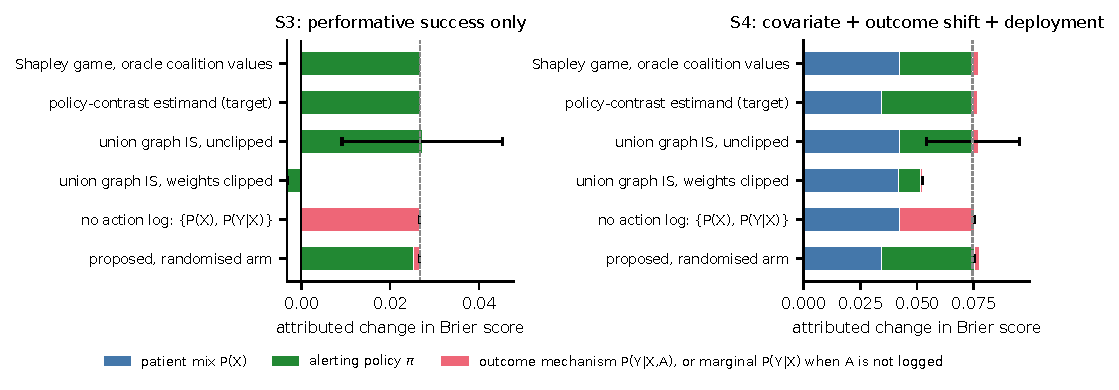
\includegraphics[width=\textwidth]{figures/fig1_attribution.pdf}
\caption{Attribution of the Brier-score change under S3 and S4, two references
and four estimators (mean over 30 seeds; error bar on the unclipped estimator
is one SD of its policy term). Dashed line: total change.}\label{fig:attr}\end{figure*}
\begin{figure*}[t]\centering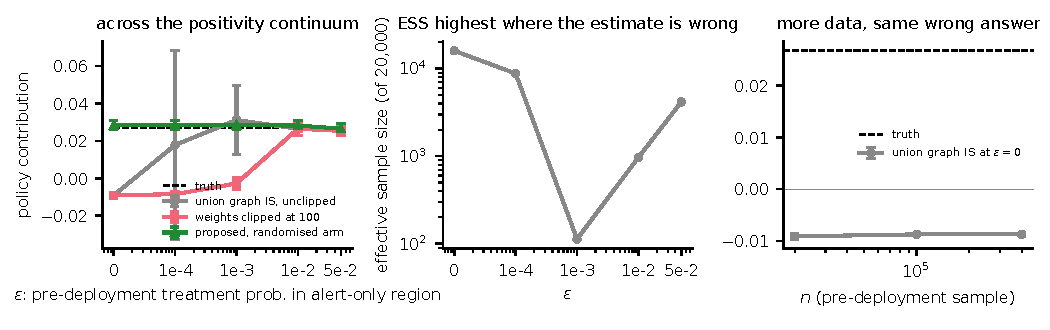
\includegraphics[width=\textwidth]{figures/fig2_positivity.pdf}
\caption{The positivity continuum. Left: policy contribution by estimator as
the pre-deployment treatment probability in the alert-only region varies.
Middle: effective sample size of the policy weights. Right: at
$\varepsilon = 0$ the bias of the union-graph estimator is constant in $n$ while
its standard error shrinks.}\label{fig:positivity}\end{figure*}
\begin{figure*}[t]\centering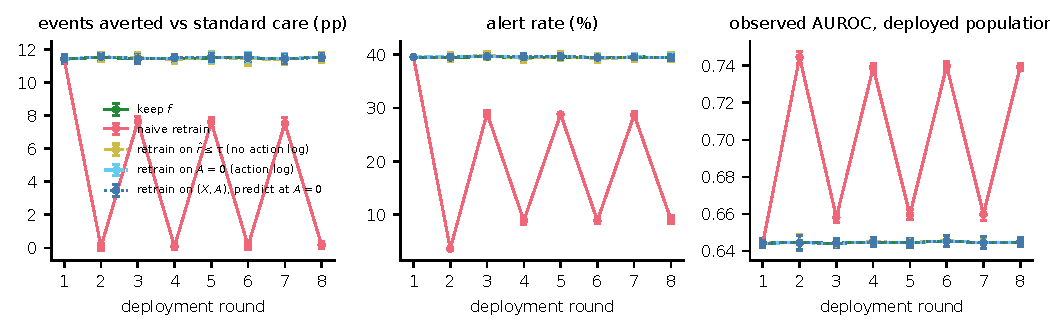
\includegraphics[width=\textwidth]{figures/fig3_retrain.pdf}
\caption{Five update rules with the original alert rate held on independent
calibration patients. Each panel shows expected events averted versus its
scenario-specific standard care, on a shared vertical scale. Left:
$\kappa=0$; right: $\kappa=2$. Twenty independent seeds per panel, eight
rounds, and matched patient draws across rules within each seed. Shading gives
$1.96$ Monte Carlo SEs of the across-seed mean. The dashed horizontal line is
standard care.}\label{fig:retrain}\end{figure*}
\begin{figure*}[t]\centering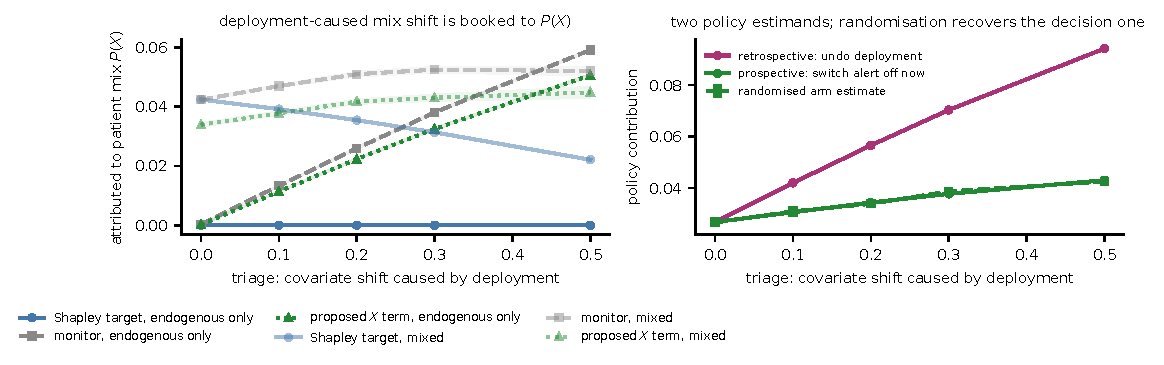
\includegraphics[width=\textwidth]{figures/fig4_triage.pdf}
\caption{Deployment-caused covariate shift (triage). Left: attribution to
$P(X)$ by the truth, the monitor and the proposed $X$ term. Right: retrospective
and prospective policy contrasts and the randomised-arm estimate.}\label{fig:triage}\end{figure*}
\begin{figure*}[t]\centering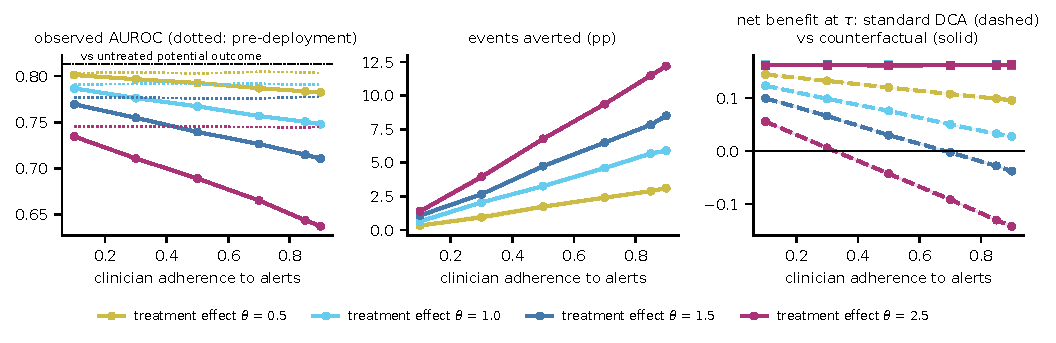
\includegraphics[width=\textwidth]{figures/fig5_utility.pdf}
\caption{Observed AUROC, events averted, and standard versus counterfactual net
benefit across clinician adherence and treatment effect.}\label{fig:utility}\end{figure*}

\section{Related work}
\label{sec:related}

\todo{Half a page, third person throughout. Attribution:
\citep{zhang2023attributing} (ICML 2023), \citep{budhathoki2021rootcauses}
(AISTATS 2021), \citep{cai2023disde}, \citep{gordaliza2025causal} (MedEurIPS 2025
workshop). Performativity: \citep{perdomo2020performative},
\citep{kabra2024limitations} (ICML 2024 workshop), \citep{lee2026partially}.
Prediction under interventions: \citep{sperrin2018msm},
\citep{vangeloven2020prediction}, \citep{lin2021scoping}, \citep{keogh2024prediction},
\citep{luijken2024estimands}. Victims of their own success:
\citep{lenert2019victims}, \citep{sperrin2019explicit}, \citep{balcarcel2025feedback}.
Monitoring and governance that detect or regulate updates without attributing:
\citep{wu2024regulating} (CHIL 2024), \citep{gonzalez2025regulating},
\citep{afdideh2026aegis}, \citep{domainsat2026}.}

%==============================================================================
\section{Limitations and responsible-use statement}
\label{sec:responsible}

\todo{Required by the workshop; a missing statement is grounds for desk
rejection. Half a page.}

\paragraph{Limitations.} Results are theoretical and synthetic; no real
deployment logs are analysed. The decomposition is order-dependent in its
split of interaction terms. The RD result identifies a local effect; the global
policy term is bounded, not pointed, without homogeneity.

\paragraph{Responsible use.} From routine observational post-deployment data,
model-mediated improvement is not identifiable; any attribution produced
without a source of identifying variation is a sensitivity analysis, not
evidence. Misattribution has a concrete clinical cost in both directions:
attributing performative success to outcome-mechanism shift retrains an
effective model and removes its benefit; attributing a genuine outcome shift to
the model's success leaves a degraded model in place. The method requires
logging of alert exposure and action, which has privacy and workflow
implications that should be governed under existing post-market surveillance
frameworks~\citep{gonzalez2025regulating}. Nothing here should be read as
supporting the deployment or retention of a model without prospective
evaluation of patient outcomes.

% bibliography style is set by aaai2026.sty
\bibliography{references}

\appendix
\section{Threshold-discontinuity experiment}
\label{app:rd}
\todo{Figure and text for the RD experiment (merged\_expE): local jump, effect curve, bounds; ITT scale; dilution by treated suspicious patients below the threshold.}

\section{Robustness of Experiments A and B}
\label{app:robustness}
The deployed score remains logistic-linear. Additional covariates enter the
linear score, and in the misspecified cells the true outcome logit also includes
$0.65\{X_1X_3+0.3(X_3^2-1)\}$. Experiment A repeats S1--S4; Experiment B
repeats the positivity continuum and an independent sample-size sweep at
$\varepsilon=0$. Each row uses an independent seed block, 12 replications of
$12{,}000$ patients per environment, and a $120{,}000$-patient oracle reference.

\begin{table}[h]
\centering\scriptsize
\caption{S3 attribution and $\varepsilon=0$ bias. The union-graph bias at
$n=96{,}000$ is relative to its oracle Shapley target. Its Monte Carlo SE is
at most $0.00013$ across 12 independent seeds. All values are Brier units.}
\label{tab:robustness}
\resizebox{\columnwidth}{!}{%
\begin{tabular}{lrrrr}
\toprule
Setting & True $\Delta R$ & Naive $Y|X$ & E3 $\pi$ & Union bias\\
\midrule
$d=10$, linear  & 0.03134 & 0.03101 & 0.03099 & $-0.03957$\\
$d=10$, nonlinear & 0.02803 & 0.02645 & 0.02827 & $-0.03644$\\
$d=20$, linear  & 0.03108 & 0.03062 & 0.03153 & $-0.04005$\\
$d=20$, nonlinear & 0.02860 & 0.02789 & 0.02898 & $-0.03619$\\
\bottomrule
\end{tabular}
}
\end{table}
F1 survives in all four settings: with no action player, nearly the entire S3
change is booked to the marginal outcome mechanism. F2 also survives: the
$\varepsilon=0$ union-graph bias remains between $-0.036$ and $-0.040$ as
sample size rises from $6{,}000$ to $96{,}000$; the full independent-seed
sweeps and all S1--S4 results are in \texttt{merged\_expAB\_robustness.json}.

\section{Persistent-site stepped wedge}
\label{app:sites}
Experiment G2 follows 48 sites for six periods. Sites cross at periods 2--5;
the period-5 cohort supplies not-yet-deployed controls for the earlier three
crossovers. The recorded site characteristic affects case mix and baseline
outcome risk. In two settings it also affects rollout priority, and in one of
those it affects the site-specific covariate trend. A crossover difference in
differences estimates the retrospective Brier term and separates changes in
the first-two-coordinate mean of $X$ into a common trend and a deployment
increment. For Brier-scale $X$ terms, an additional estimator reweights
observed pre-rollout losses under a Gaussian location shift, with site means
and covariance estimated from observed covariates. Simulator counterfactuals
are used only to measure bias.
With random rollout order, retrospective bias is $-0.00075$ (Monte Carlo SE
$0.00038$). Characteristic-linked order with a common covariate trend yields
$-0.00535$ ($0.00033$), even though the estimated covariate-mean split is
nearly unbiased. When site-specific trends also follow the characteristic,
retrospective bias is $-0.00267$ ($0.00044$), and the induced and exogenous
covariate-mean biases are $+0.04311$ and $-0.04229$. These results concern the
supported crossover cohorts. They do not identify the final cohort's effect
without an additional control period or assumption.
The Brier-scale $X$ split has its own estimator error: the induced and
exogenous components have biases $-0.00209$ and $+0.00237$ with random order,
and $+0.00107$ and $-0.00087$ with characteristic-linked order and site trends.
Random rollout does not remove the finite-sample and location-model error of
this reweighting step.

\section{Proofs}
\todo{Proposition~\ref{prop:absence}: exhibit $x, a$ with support mismatch;
show the hybrid requires an undefined conditional; conclude non-identification.
Proposition~\ref{prop:misattr}: with $P(X)$ unchanged, $v(\{P(X)\}) = 0$ and
$v(\{P(Y|X)\}) = v(\mathcal{M}') = \Delta R$, so Shapley values follow by
efficiency. Proposition~\ref{prop:rd}: write $\Delta_\pi = \int_\tau^1
\theta(r)\, dP(\rhat = r)$ and bound.}

\end{document}
